\section{Modular graphs}
We consider a modular graph with 64 nodes and four modules,
denoted as $\mathcal{G}^{(64, p_1, p_2)}_{\mathsf{M}}$, in which $p_1 = 0.01$, and $p_2 = 0.5$,
where $p_1$ is the probability that a particular node of a given module is connected to any other node of a different module,
and $p_2$ is the probability that a particular node is connected to any other node of the same module.

On what concerns hyperparameter tunning, we fix $\beta = 4$ for all values of $T/N$.

Figure~\ref{fig:performance-modular} shows the performance of the proposed algorithms and
the benchmarks. As we can note, the \textsf{SGL} algorithm outperforms the \textsf{CGL} algorithm
in terms of F-score, while having a comparable performance in terms of relative error.

\begin{figure}[!htb]
    \centering
    \begin{subfigure}[b]{0.47\textwidth}
      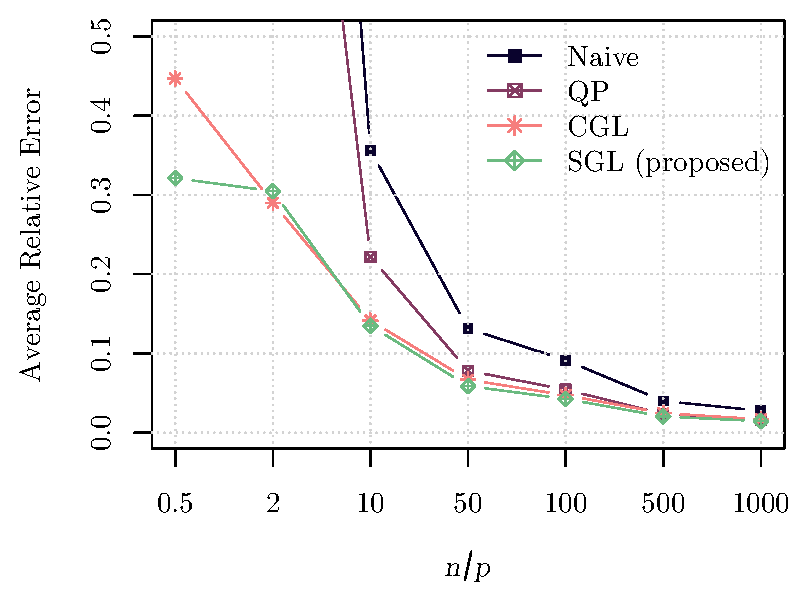
\includegraphics[width=\textwidth]{modular/latex/figures/relative_error_modular.eps}
    \end{subfigure}
    ~ %add desired spacing between images, e. g. ~, \quad, \qquad, \hfill etc.
      %(or a blank line to force the subfigure onto a new line)
    \begin{subfigure}[b]{0.47\textwidth}
        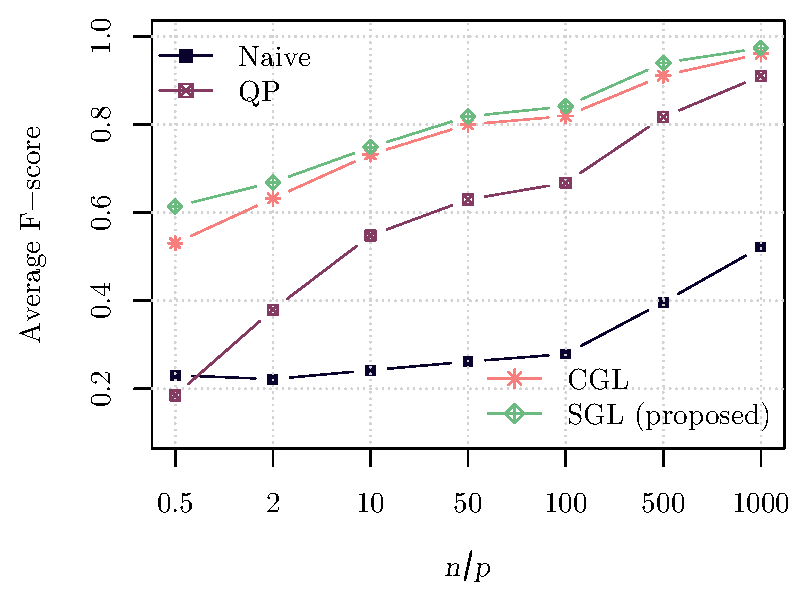
\includegraphics[width=\textwidth]{modular/latex/figures/fscore_modular.eps}
    \end{subfigure}
    \caption{Average performance results for learning Laplacian matrix of a $\mathcal{G}^{(64, 0.01, 0.5)}_{\mathsf{M}}$
    with four modules.}
    \label{fig:performance-modular}
\end{figure}

